\documentclass{beamer}
\usepackage[utf8]{inputenc}
\usepackage{graphicx}

% Theme
\usetheme{Ilmenau}
%\usetheme{Warsaw}
%\usecolortheme{beaver}
\setbeamertemplate{headline}{} 

% Commands
\newcommand{\fx}{\emph{JavaFX} }
\newcommand{\java}{\emph{Java} }
\newcommand{\fxml}{\emph{FXML} }
\newcommand{\himalaya}{\emph{Himalaya} }
\newcommand{\reference}[1]{(Voir Figure \ref{fig:#1},  page \pageref{fig:#1}) }

\begin{document}
	\title{\textbf{Projet Himalaya}}
	\subtitle{Soutenance de projet\\
		{\footnotesize M1 ISIDIS}}
	\author {Alexis Jouin et Sébastien Schouteeten}
	\institute{
\includegraphics[height=3cm]{images/ulco}}
	\date{Années 2016 -- 2017}
	\frame[plain]{
		\titlepage
	}
	
	\institute{Université du Littoral Côte d'Opale}
	
	\section{Plan}
	\begin{frame} 
		\frametitle{Plan}
		\tableofcontents
	\end{frame}

	\section*{Introduction}
	\begin{frame}
		\frametitle{Introduction}
		
		\begin{block}{Projet de fin d'année}
			\begin{itemize}
			\item Projet Master ISIDIS
			\item Binôme : Alexis Jouin et Sébastien Schouteeten
			\item Initiation pour un projet de recherche	
			\end{itemize}
		\end{block}
	
		\begin{block}{But du projet}		
			Développer un bot en \java pour un jeu de société \himalaya		
		\end{block}
	
		\begin{alertblock}{Problématiques}
			\begin{itemize}
				\item Quel algorithme est le mieux adapté pour le jeu \himalaya ?
				\item Comment l'implémenter ?
				\item Quels sont les paramètres à varier ?
			\end{itemize}
		\end{alertblock}
	
	\end{frame}
	
	
\section*{Plan}
	\begin{frame} 
		\frametitle{Plan}
		\tableofcontents
	\end{frame}

	\section{Présentation du projet}
	\begin{frame}
		\frametitle{Présentation}
		\begin{block}{Le projet}
			\begin{itemize}
				\item Moteur existant de l'ancien projet de \emph{l'Université de Nice} mais pas d'interface graphique
				\item Création de l'interface graphique avec \fx
				\item Recréer le moteur pour meilleur adaptation avec \fx
				\item Toutes les ressources (images) ont étaient reprises de l'ancien projet
				\item Développer l'intelligence artificielle
			\end{itemize}
		\end{block}	
\end{frame}
	
	\section{Les règles du jeu}

	\begin{frame}
	\frametitle{Les règles du jeu}
	\framesubtitle{Descriptif du jeu}
	
	\begin{block}{Le jeu}
		\begin{itemize}
			\item Jeu de société
			\item Jeu de plateau stratégique avec planification des actions
		\end{itemize}
	\end{block}
	
	\begin{block}{Résumé des règles}
		\begin{itemize}
			\item 20 villages avec des ressources et des commandes sur certains
			\item Les joueurs choisissent leur village de départ
			\item À chaque tour, planifier 6 actions afin de pouvoir récupérer des ressources et honorer des commandes
			\item Après chaque commande honorée, 2 récompenses parmi 3
			\item Les récompenses permettent d'augmenter le score économique, politique ou religieux
		\end{itemize}
	\end{block}
	
	\end{frame}


	\begin{frame}
		\frametitle{Les règles du jeu}
		\framesubtitle{Éléments du jeu sur le plateau}
		
		\begin{figure}[h]
		\centering
		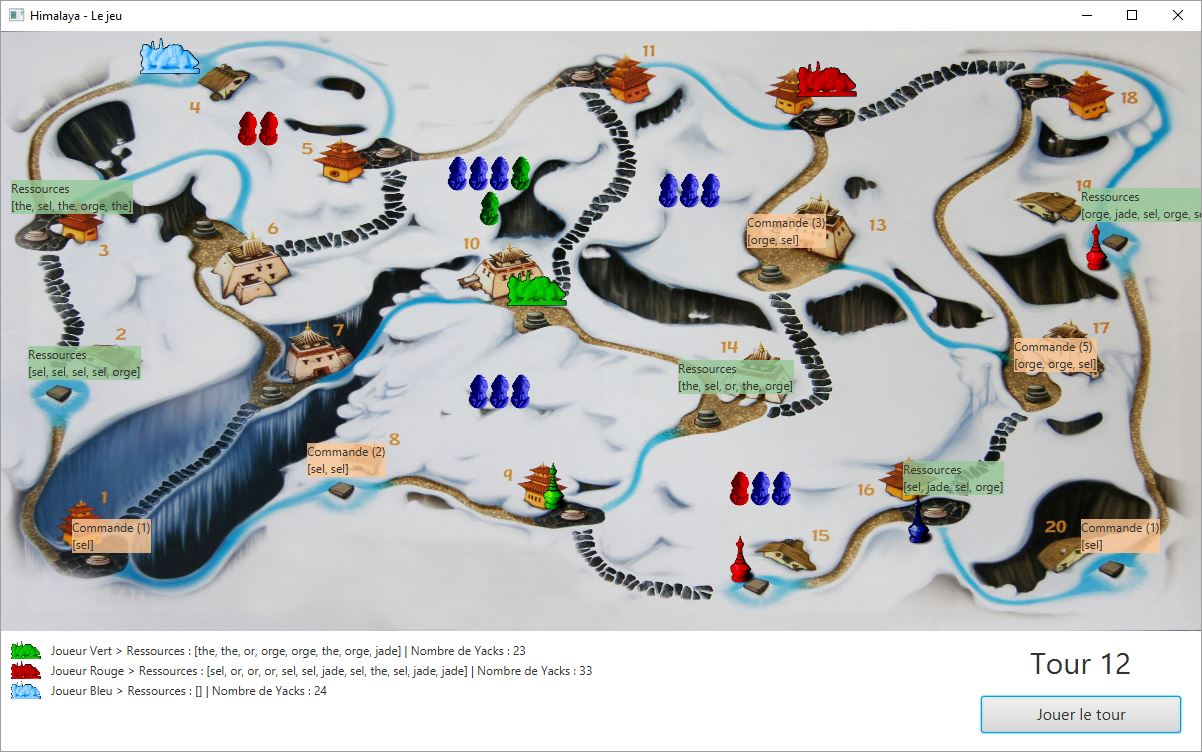
\includegraphics[width=1\linewidth]{images/etat_jeu_avance}
		\caption{Plateau du jeu durant la partie}
		\label{fig:plateau}
		\end{figure}
	
	\end{frame}


	
	% !TeX spellcheck = fr_FR
\section{Développement du moteur et de l'interface}
	\begin{frame}
		\frametitle{Développement du moteur et de l'interface}
		\framesubtitle{Le moteur du jeu}
		\begin{figure}[h]
			\centering
			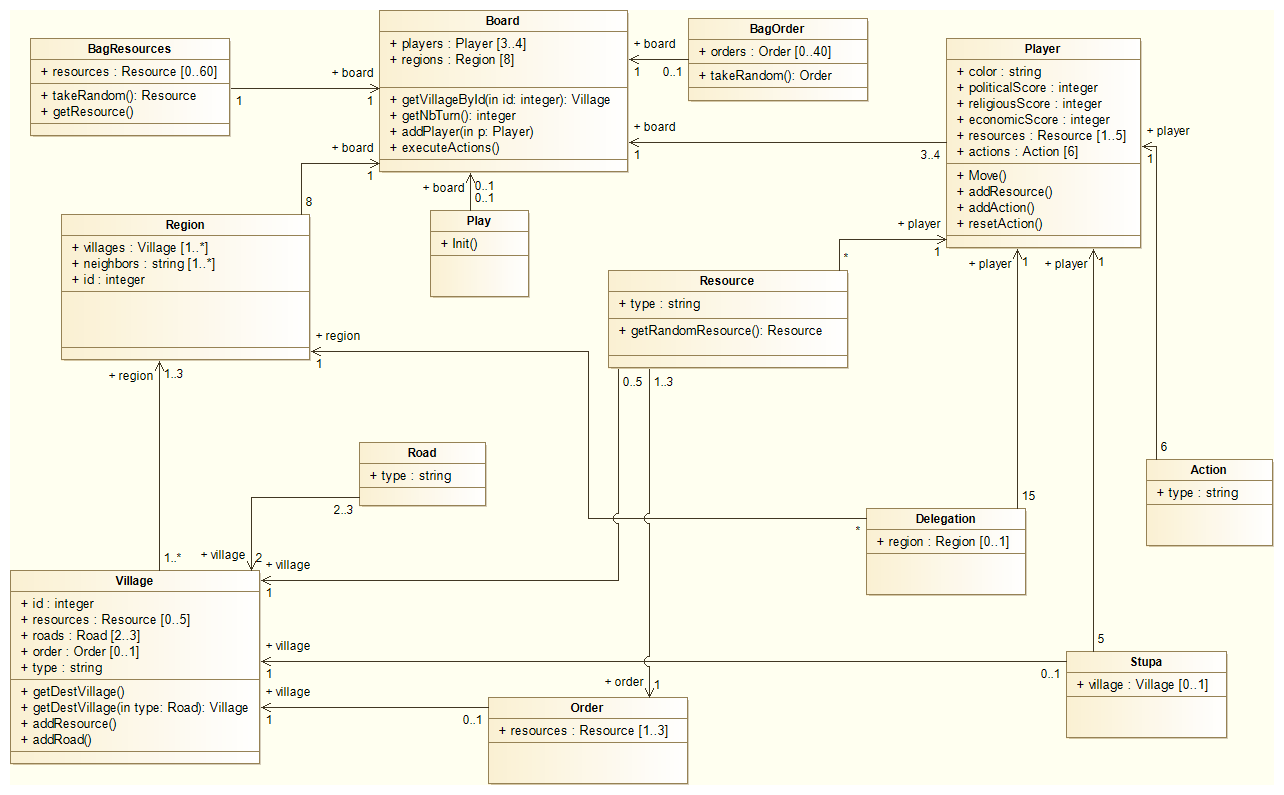
\includegraphics[width=0.8\linewidth]{images/UML_Himalaya_2}
			\caption{UML créé avant le développement}
			\label{fig:uml}
		\end{figure}
		
	\end{frame}

	\begin{frame}
		\frametitle{Développement du moteur et de l'interface}
		\framesubtitle{Le moteur du jeu}
		\begin{figure}[h]
			\centering
			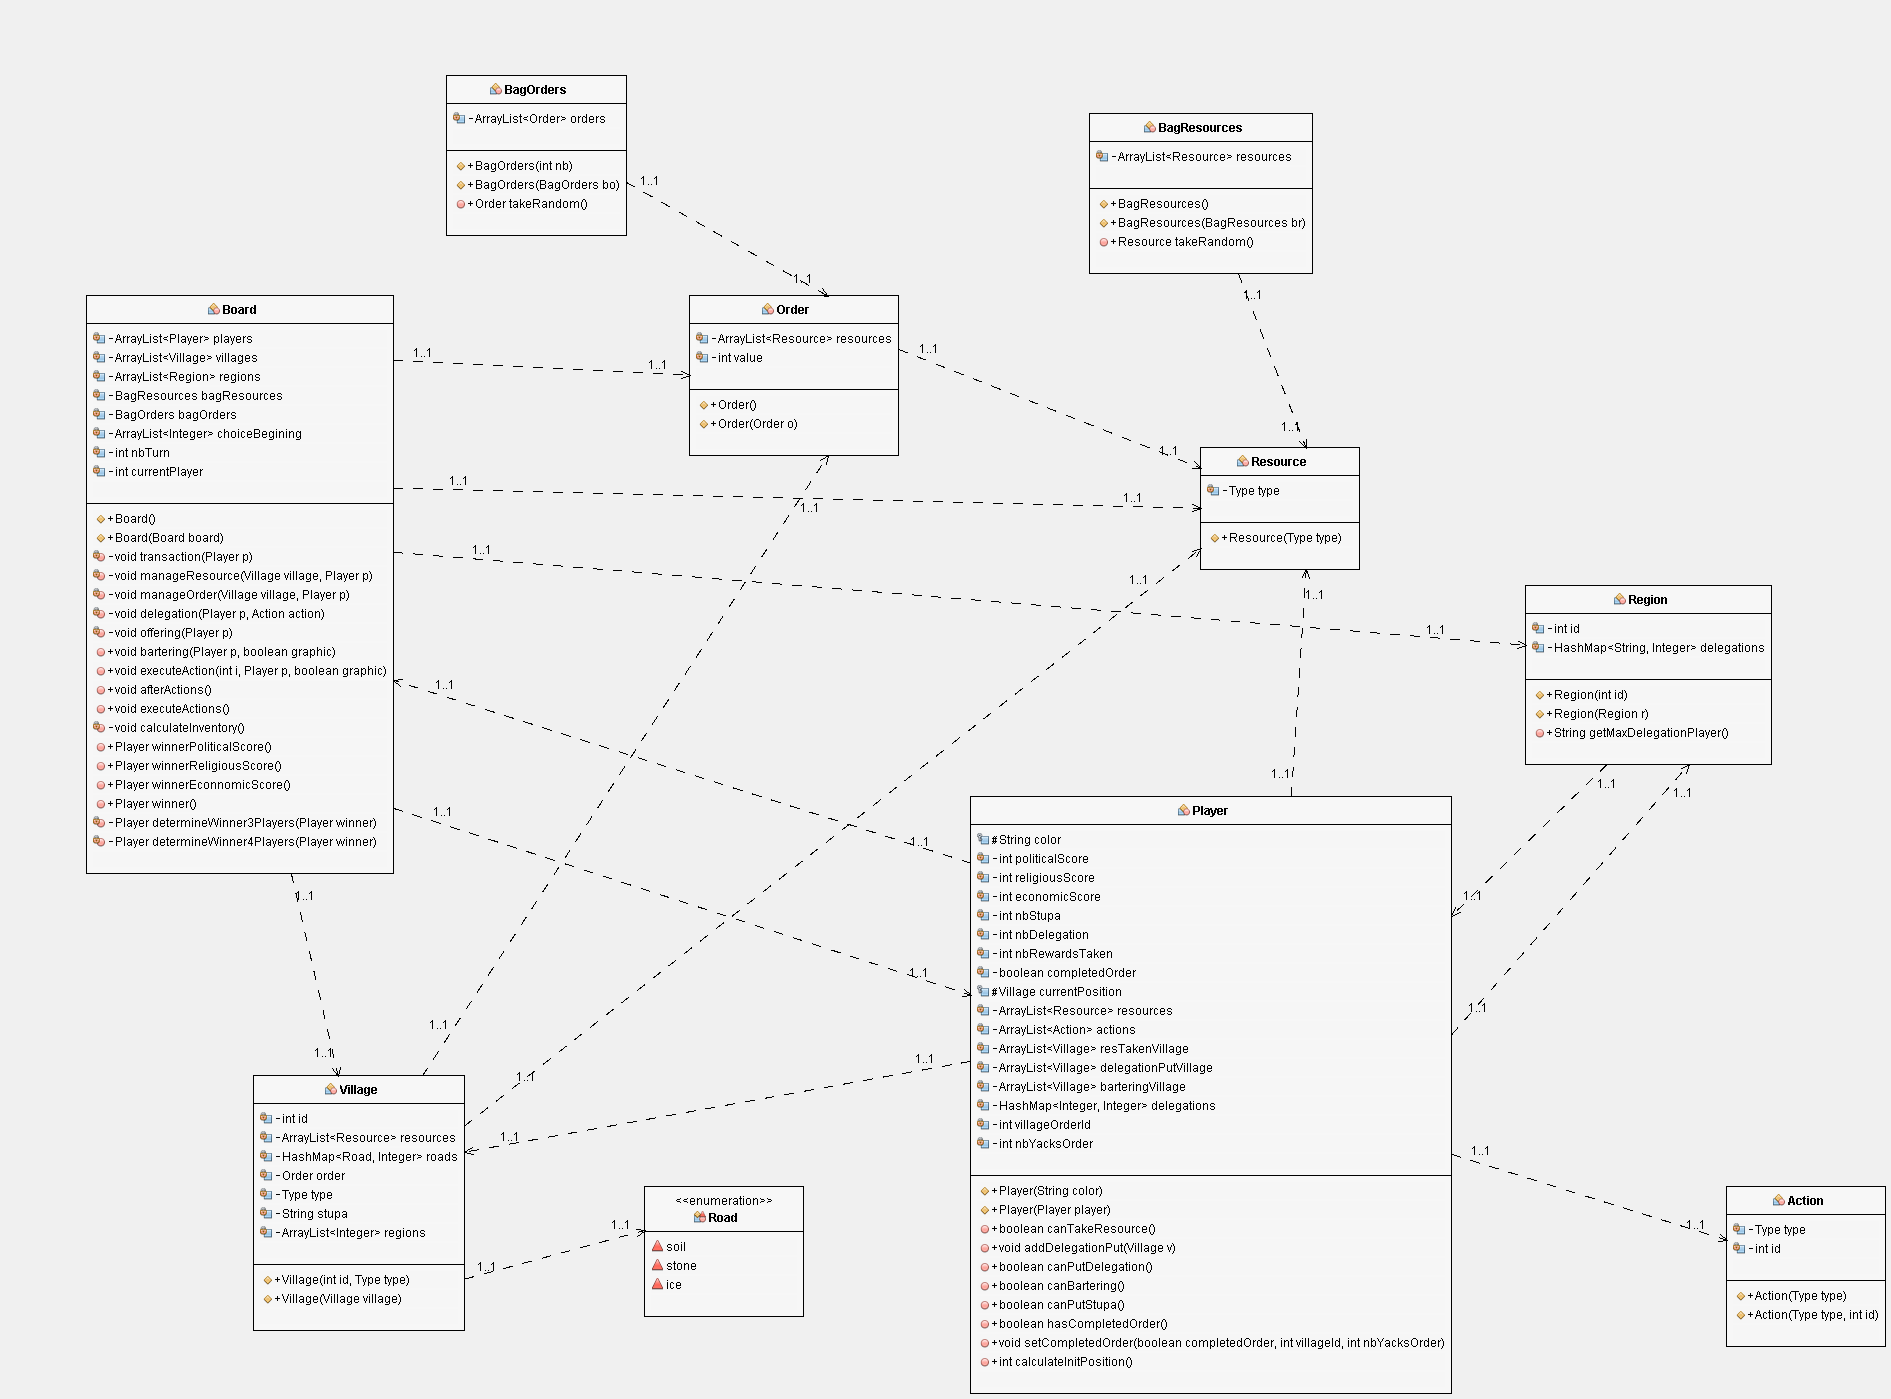
\includegraphics[width=0.8\linewidth]{images/UML_Himalaya_CORE_3}
			\caption{UML généré après le développement}
			\label{fig:uml}
		\end{figure}
	\end{frame}

	\begin{frame}
		\frametitle{Développement du moteur et de l'interface}
		\framesubtitle{Le moteur du jeu}
		\begin{block}{Le moteur}
			\begin{itemize}
				\item Utilisable pour version Graphique et Console
				\item Tests unitaires
				\item Classe Player avec classes fille IA
			\end{itemize}
		\end{block}	
	\end{frame}

	\begin{frame}
		\frametitle{Développement du moteur et de l'interface}
		\framesubtitle{L'interface graphique du jeu}
		\begin{block}{\fx}
			\begin{itemize}
				\item Pour chaque page : fichier \fxml et Controller 
				\item Création d'un "Framework" pour navigation entre les pages
				\item Utilisation du "Scene Builder" avec NetBeans
			\end{itemize}
		\end{block}	
	\end{frame}
	
	\begin{frame}
		\frametitle{Développement du moteur et de l'interface}
		\framesubtitle{L'interface graphique du jeu}
		\begin{figure}[h]
			\centering
			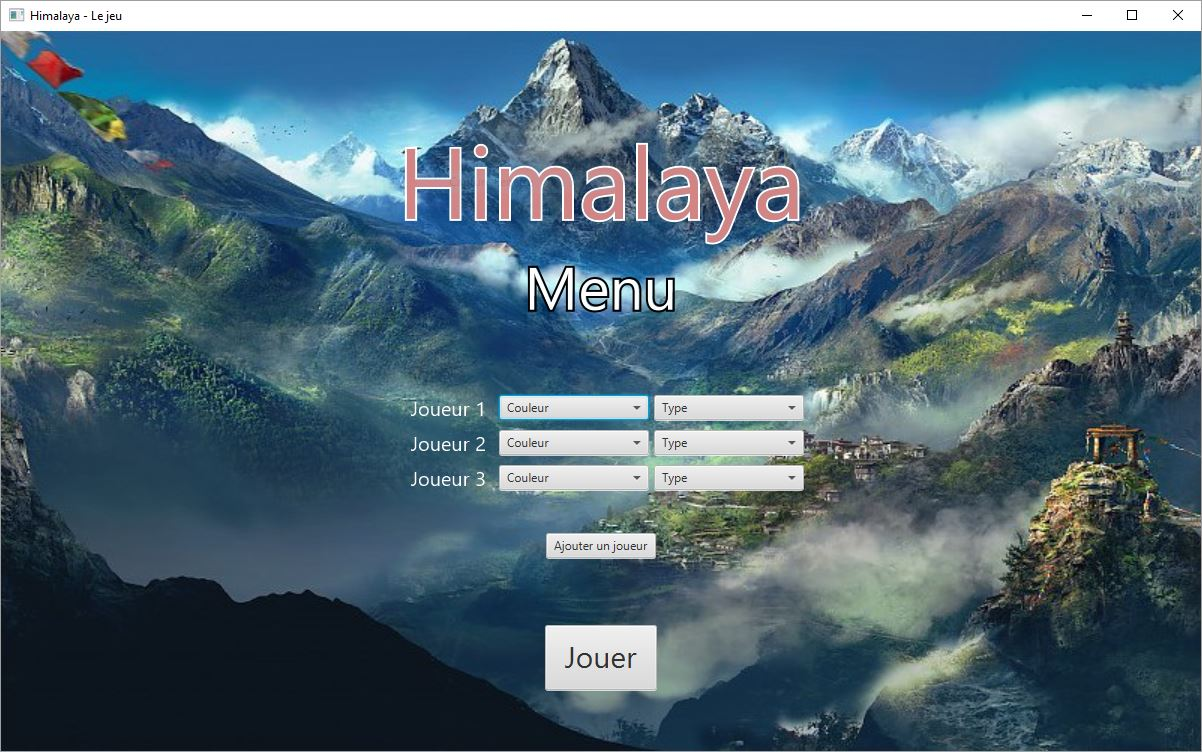
\includegraphics[width=0.8\linewidth]{images/menu}
			\caption{Menu du jeu}
			\label{fig:menu}
		\end{figure}
	\end{frame}
	
	\begin{frame}
		\frametitle{Développement du moteur et de l'interface}
		\framesubtitle{L'interface graphique du jeu}
		\begin{figure}
			\begin{subfigure}{0.5\textwidth}
				\centering
				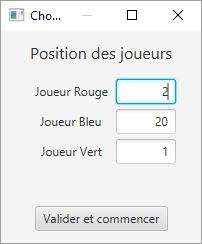
\includegraphics[width=0.4\linewidth]{images/position}
				\caption{Position Joueur}
				\label{fig:position}
			\end{subfigure}
			\begin{subfigure}{0.4\textwidth}
				\centering
				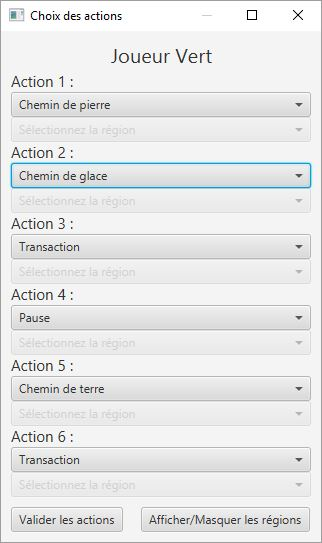
\includegraphics[width=0.5\linewidth]{images/actions}
				\caption{Fenêtre des actions}
				\label{fig:actions}
			\end{subfigure}
		\end{figure}
	\end{frame}

	\begin{frame}
		\frametitle{Développement du moteur et de l'interface}
		\framesubtitle{L'interface graphique du jeu}
		\begin{figure}[h]
			\centering
			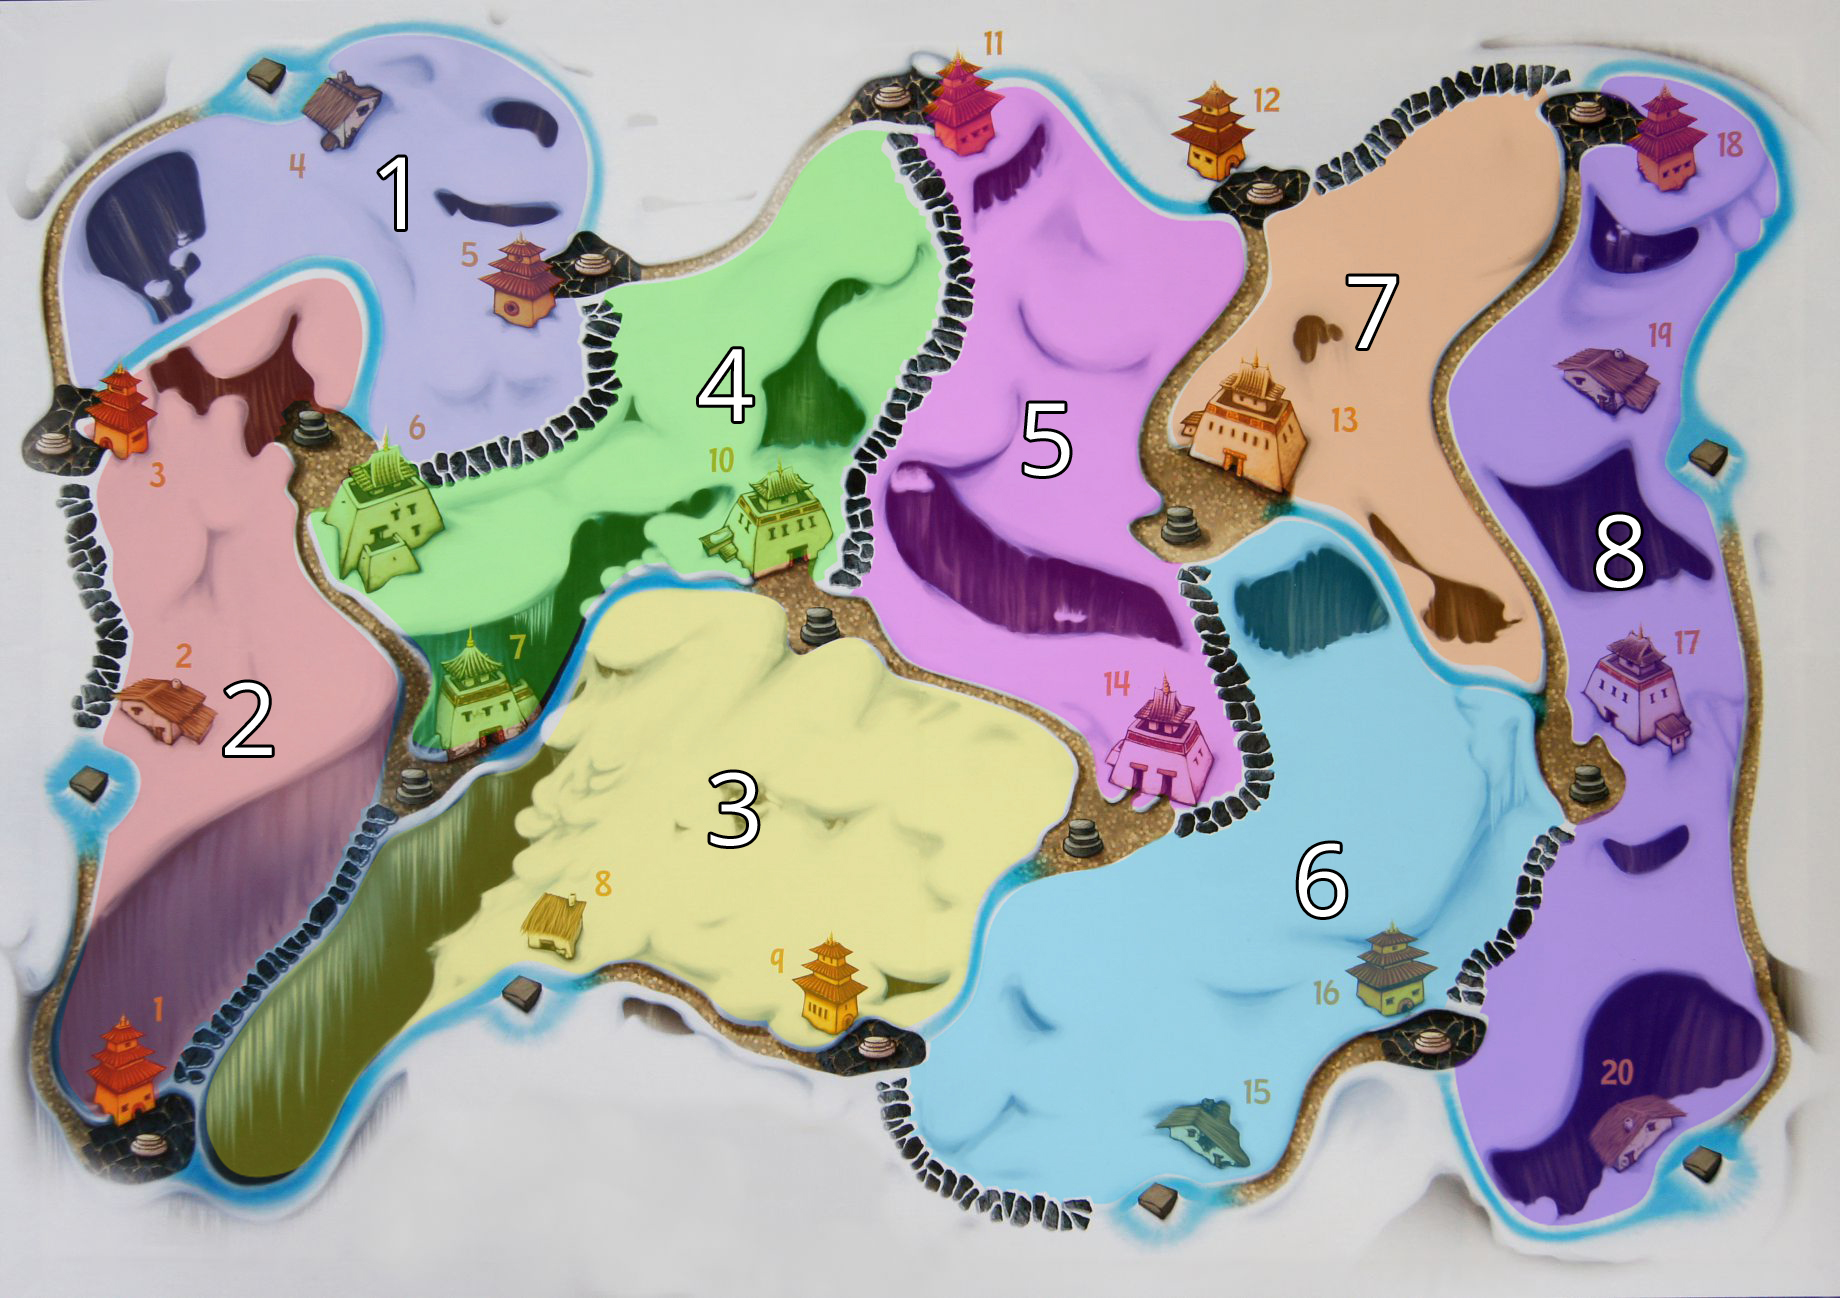
\includegraphics[width=0.8\linewidth]{images/board_regions}
			\caption{Régions sur le plateau}
			\label{fig:regions}
		\end{figure}
	\end{frame}

	\begin{frame}
		\frametitle{Développement du moteur et de l'interface}
		\framesubtitle{L'interface graphique du jeu}
		\begin{figure}[h]
			\centering
			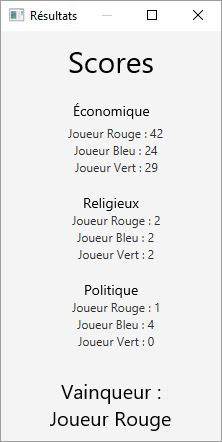
\includegraphics[width=0.25\linewidth]{images/resultats}
			\caption{Page de victoire}
			\label{fig:victoire}
		\end{figure}
	\end{frame}



	


	
	\section{L'intelligence artificielle}

\begin{frame}
	\frametitle{L'intelligence artificielle}
	\framesubtitle{Présentation de l'algorithme}
	
	\begin{block}{Les paramètres}
		\begin{itemize}
			\item Population des parents (mu) = 20
			\item Population des enfants (lambda) = 500
			\item Taille du tournoi pour la sélection = ???
			\item Taux de crossing-over = 0.8
			\item Taux de mutation = 1.0
			\item Nombre de générations maximum = 25
		\end{itemize}
	\end{block}	
	
	\begin{exampleblock}{Individu d'une population}
		\begin{itemize}
			\item Suite des 9 meilleurs actions
			\item L'IA réalise les 6 premières actions
		\end{itemize}
	\end{exampleblock}	
\end{frame}

\begin{frame}
	\frametitle{L'intelligence artificielle}
	\framesubtitle{Calcul de la fitness}
	
	\begin{block}{Calcul de la fitness}
		\begin{itemize}
			\item Copie du plateau de jeu, et de tous ses composants
			\item Pas de copie des joueurs
			\item Réalisation d'une simulation du tour pour calculer la fitness
		\end{itemize}
	\end{block}

	\begin{block}{Évaluation des coefficients}
		\begin{itemize}
			\item Coefficients égaux au départ
			\item Adaptation au score du joueur
		\end{itemize}
	\end{block}
\end{frame}

\begin{frame}
	\frametitle{L'intelligence artificielle}
	\framesubtitle{Calcul de la fitness}
	\lstinputlisting[language=Java, caption= {Pseudo-code: Calcul de la fitness}]{code/algo_fitness.java}
\end{frame}

\begin{frame}
	\frametitle{L'intelligence artificielle}
	\framesubtitle{Calcul de position et optimisation des régions}
	
	\begin{block}{Position initiale}
		\begin{itemize}
			\item Run de l'algorithme pour chaque village disponible
			\item Choisir la meilleur fitness
			\item Ajouter le village à la liste des indisponibles
		\end{itemize}
	\end{block}	
	
	\begin{exampleblock}{Région optimale des délégations}
		\begin{itemize}
			\item Liste des régions possibles
			\item Calcul de rentabilité: prise de région, vide ou occupée
			\item Prise en compte des délégations présentes du joueur
		\end{itemize}
	\end{exampleblock}	
\end{frame}
	
	\section{Résultats obtenus et perspectives}

\begin{frame}
	\frametitle{Résultats obtenus et perspectives}
	\begin{figure}[h]
		\centering
		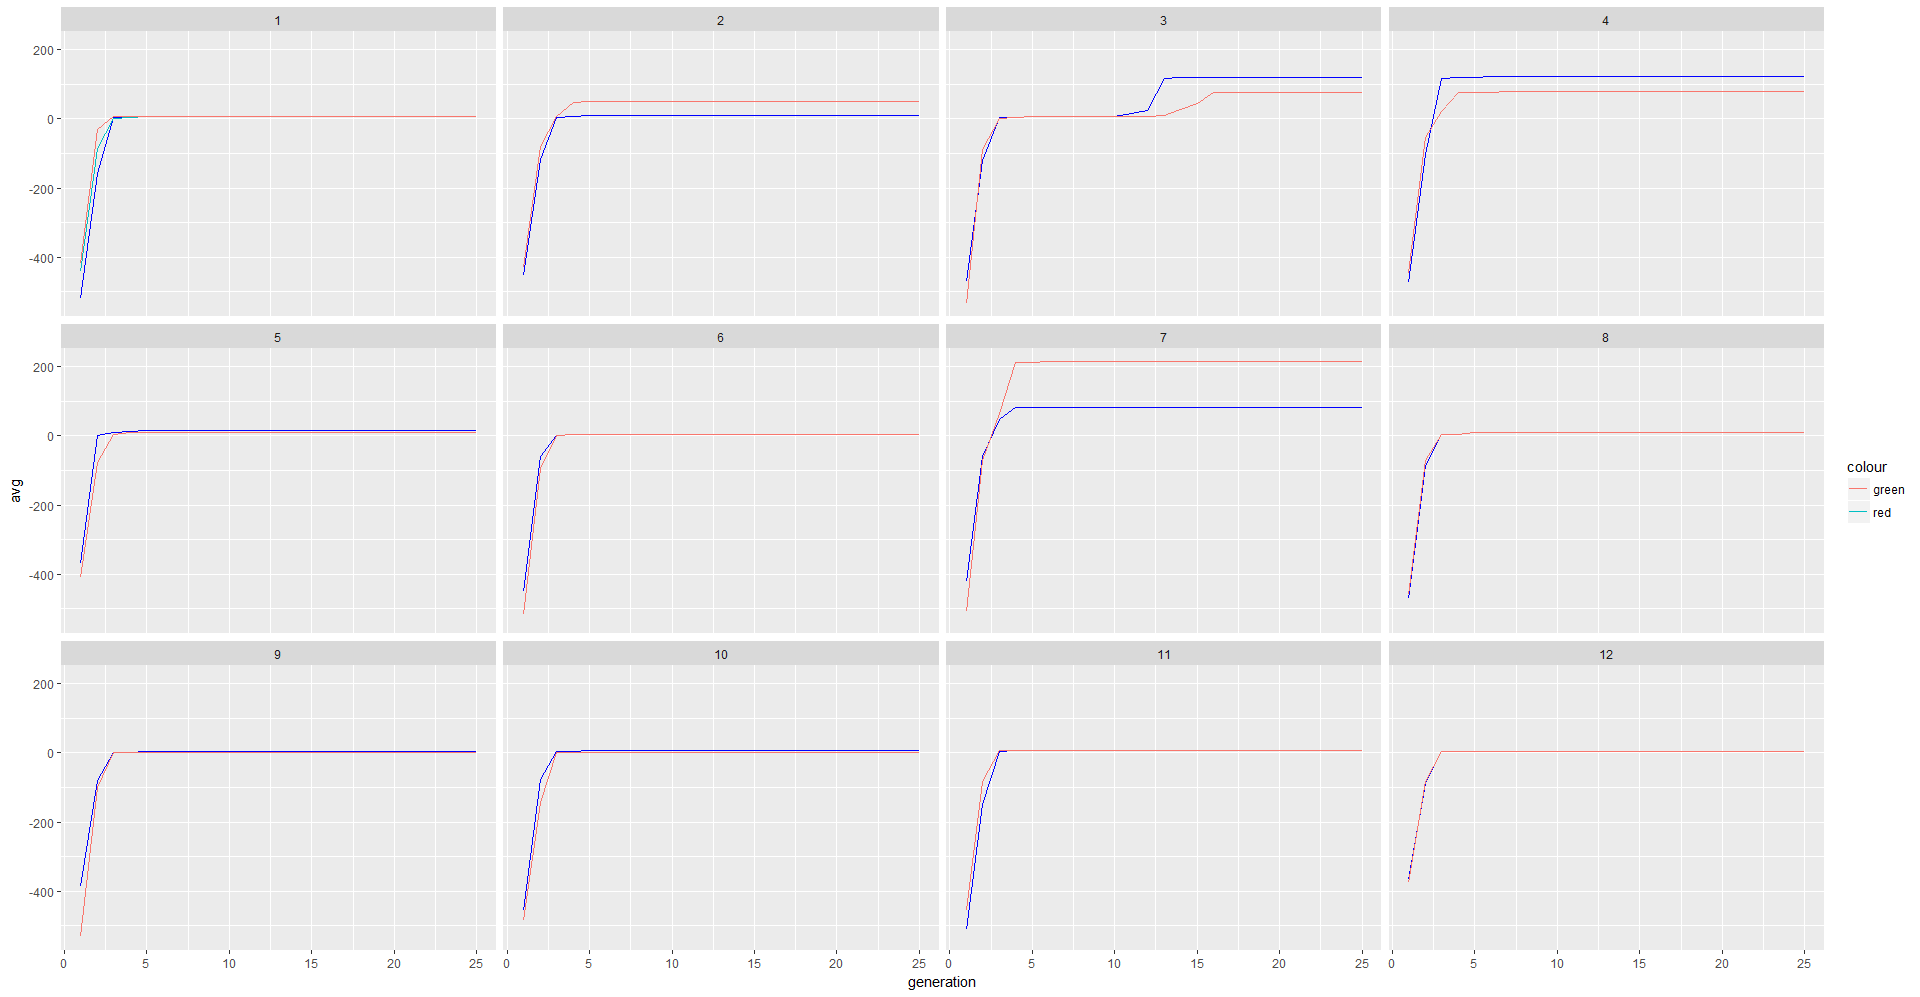
\includegraphics[width=0.8\linewidth]{images/analyseRStudio1}
		\caption{Analyse R}
	\end{figure}
\end{frame}

\begin{frame}
	\frametitle{Résultats obtenus et perspectives}
	\begin{figure}
		\begin{subfigure}{0.5\textwidth}
			\centering
			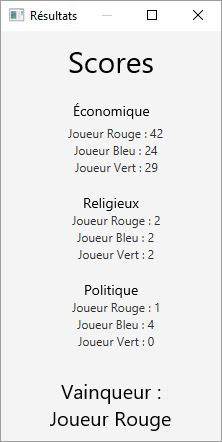
\includegraphics[width=0.4\linewidth]{images/resultats}
			\caption{3 IA évolutionnaire}
		\end{subfigure}
		\begin{subfigure}{0.4\textwidth}
			\centering
			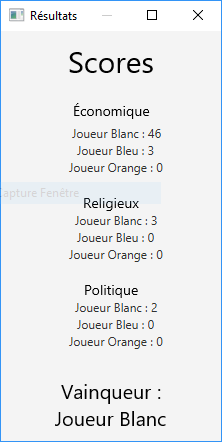
\includegraphics[width=0.5\linewidth]{images/score_evol_vs_random}
			\caption{1 IA évolutionnaire}
		\end{subfigure}
	\end{figure}
\end{frame}

\begin{frame}
	\frametitle{Résultats obtenus et perspectives}
	\begin{block}
		
	\end{block}
\end{frame}
	
	\section{Conclusion}
	\begin{frame}
	\frametitle{Conclusion et Améliorations}
	\begin{block}{Bilan}
		\begin{itemize}
			\item Application terminée et fonctionnelle avec Humain et IA
			\item L'ensemble des fonctionnalités attendues dans le cahier des charges sont respectées
			\item Travail en pair-programming, utilisation de GIT, R Studio ...
			\item Permet l'implémentation d'algorithmes vues en cours dans un projet concret
		\end{itemize}
	\end{block} 
	\begin{block}<1>{Améliorations}
		\begin{itemize}
			\item Prendre en compte les règles complexes du jeu
			\item Améliorer ou remplacer les algorithmes
			\item Algorithme génétique ?
		\end{itemize}
	\end{block} 
\end{frame}
	
\end{document}